\chapter{Product Overview}

% did the ui meet the interface requirements?
% fill inn text inbetween images
% 
% iterate on text and images

% Frempek???
This chapter describes the product as seen from a user's perspective. It focuses on giving a holistic understanding of the simulator to provide context for further chapters. DeskSim v2 as a product is a functional simulator and a building tool for the simulator. The following section will provide a representation of both the simulator and the building tool, as well as how they are presented to the user. All texts and buttons are represented in Norwegian. 

\section{Menus}

When the application is started the log in screen displays a basic user interface where the user will enter their credentials to log in and gain access to the simulator. You must be an authenticated user to use the application, since no guest mode exists. If there is an error when logging in, such as an empty field or wrong username and password, a small error text will be displayed to the user. 

\begin{figure}[H]
    \centering
    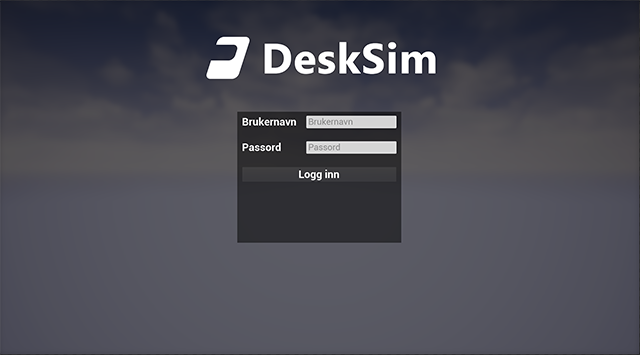
\includegraphics[width=0.8\textwidth]{figures/LogIn1.PNG}
    \caption{DeskSimV2: Log in screen}
    \label{Log_in_menu_img}
\end{figure} 


The main menu allows the user to select the level/scenario they want to run. These scenarios are separated into main categories displayed as tabs. The categories are based on the ones Lokførerskolen uses today. If the user has admin or teacher privileges they have the option to start a level/scenario in editing mode as well, as is shown with the "Editor" button in figure \ref{Main_Menu_img}.

\begin{figure}[H]
    \centering
    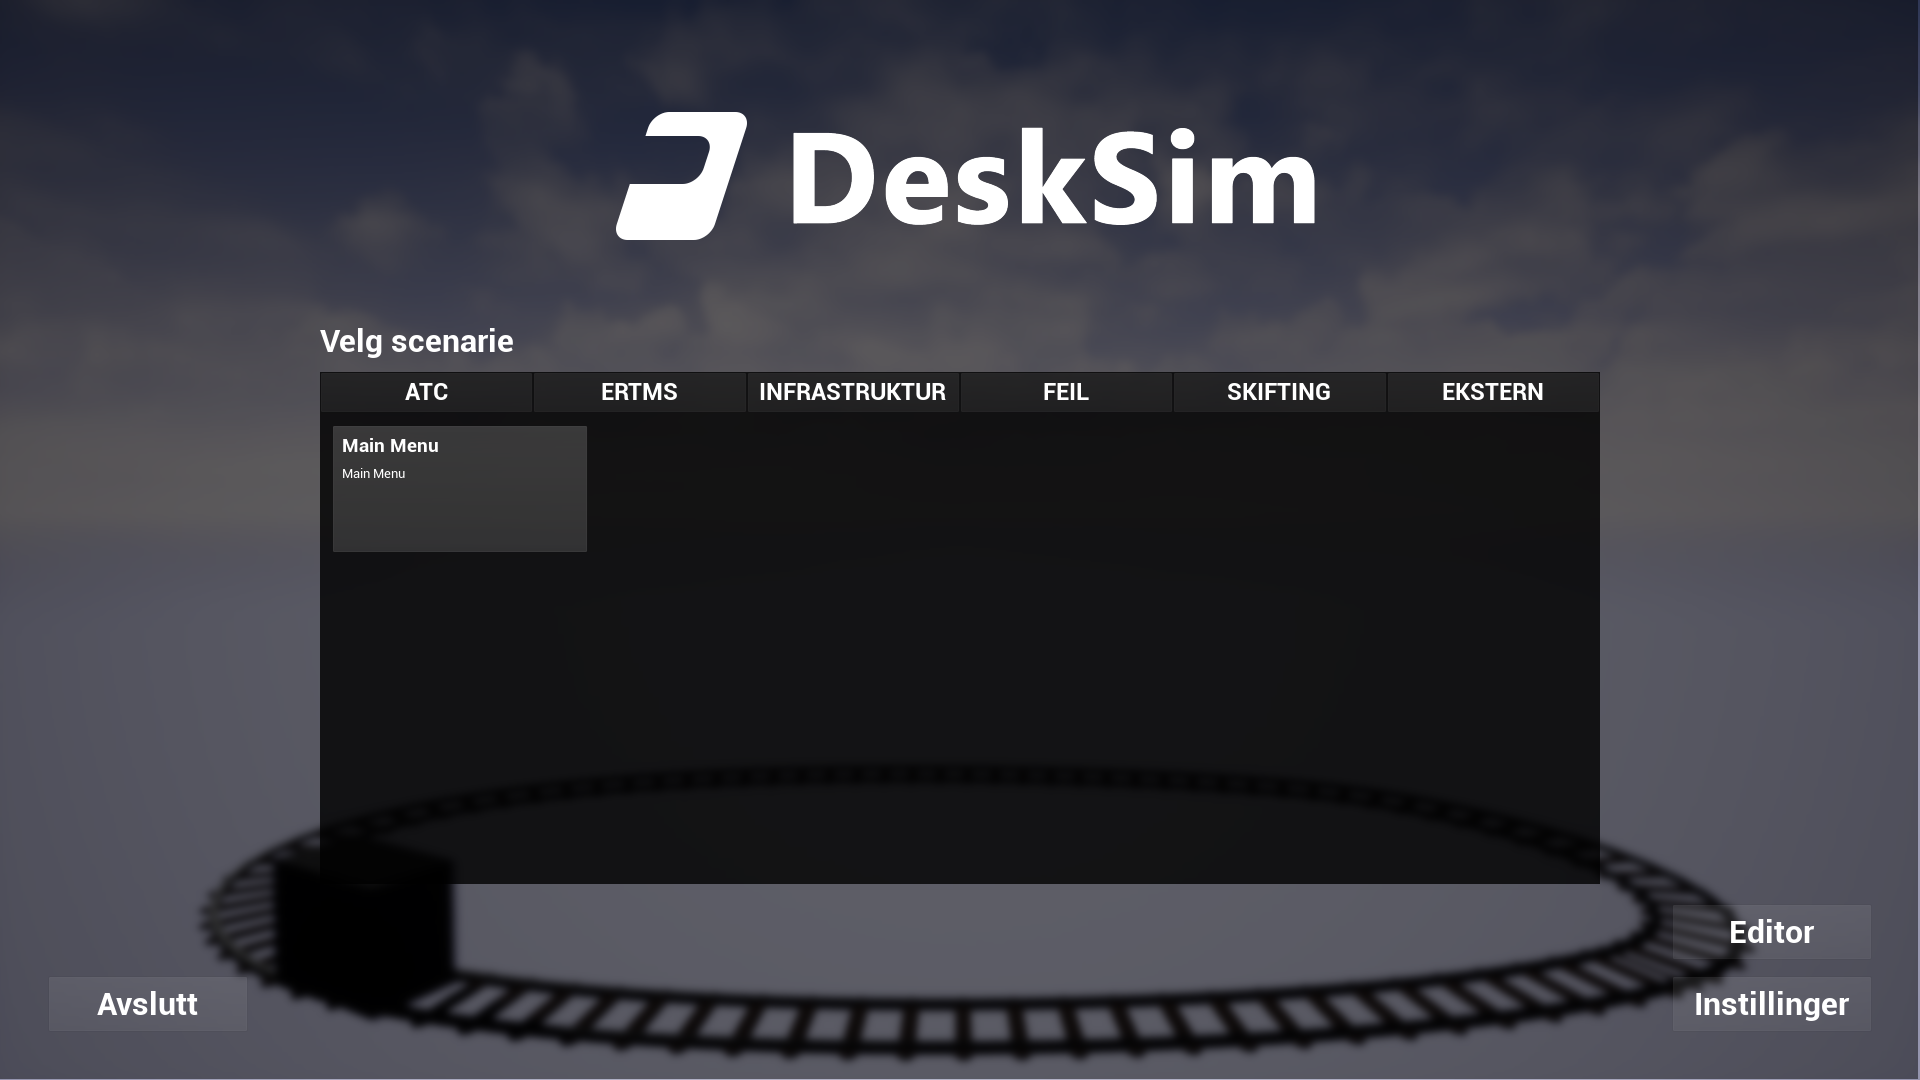
\includegraphics[width=0.8\textwidth]{figures/Main Menu.PNG}
    \vspace{12pt}
    \caption{DeskSimV2: Main Menu}
    \label{Main_Menu_img}
\end{figure} 

Pressing the "Settings" button opens up a settings menu which allows the user to change the screen resolution and the window mode for the application. This settings menu is also available in the pause menu of the game, so settings can be changed during scenarios. 

\begin{figure}[H]
    \centering
    \vspace{12pt}
    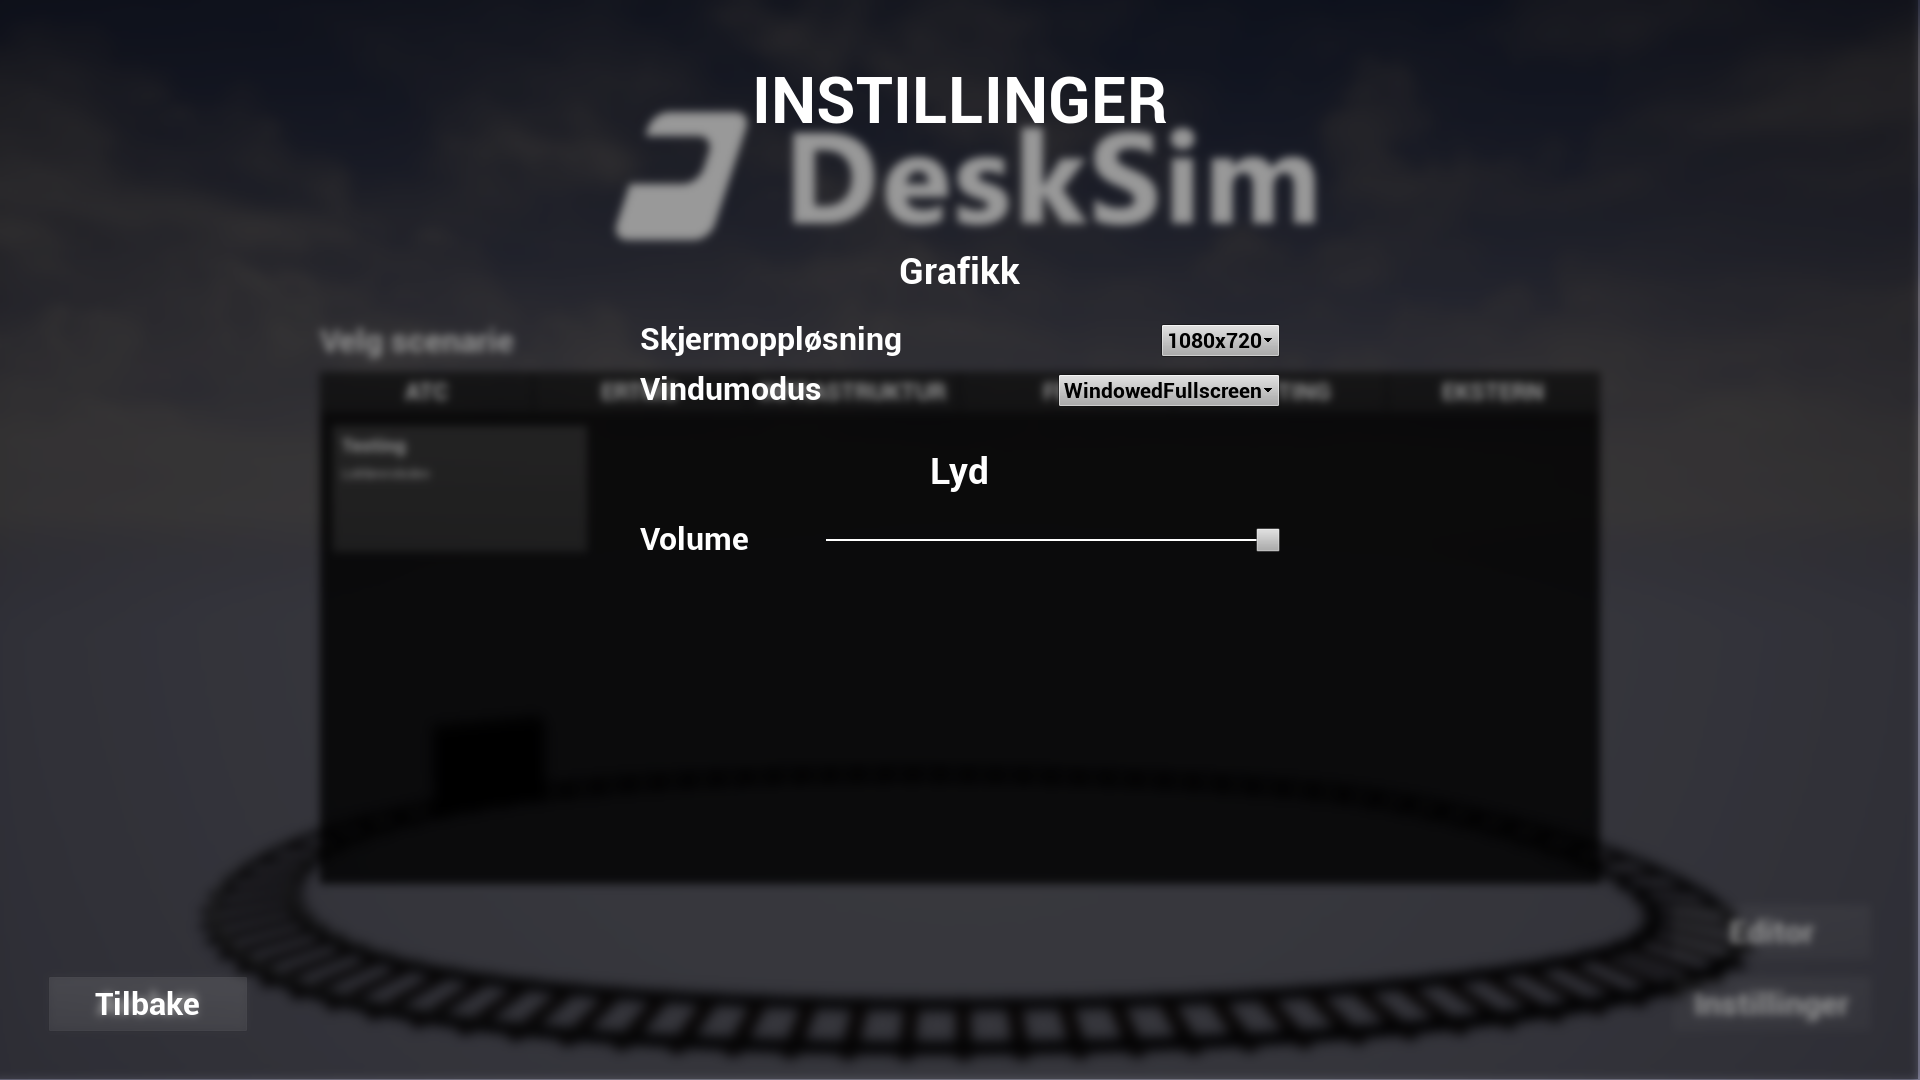
\includegraphics[width=0.8\textwidth]{figures/Settings.PNG}
    %\vspace{-12pt}
    \caption{DeskSimV2: Settings Menu}
    \label{Settings_img}
\end{figure} 

\section{Simulator mode}

The in-game experience consist of a view that corresponds to the view a train driver has from inside the front wagon of a train. The speedometer at the top left of the screen presents the user with the current speed of the train. \todo{legg til mer tekst}
%kamera ser gjennom fronten av toget, hud oppe i venstre viser fart, speedometer, osv. 

\begin{figure}[H]
    \centering
    \vspace{12pt}
    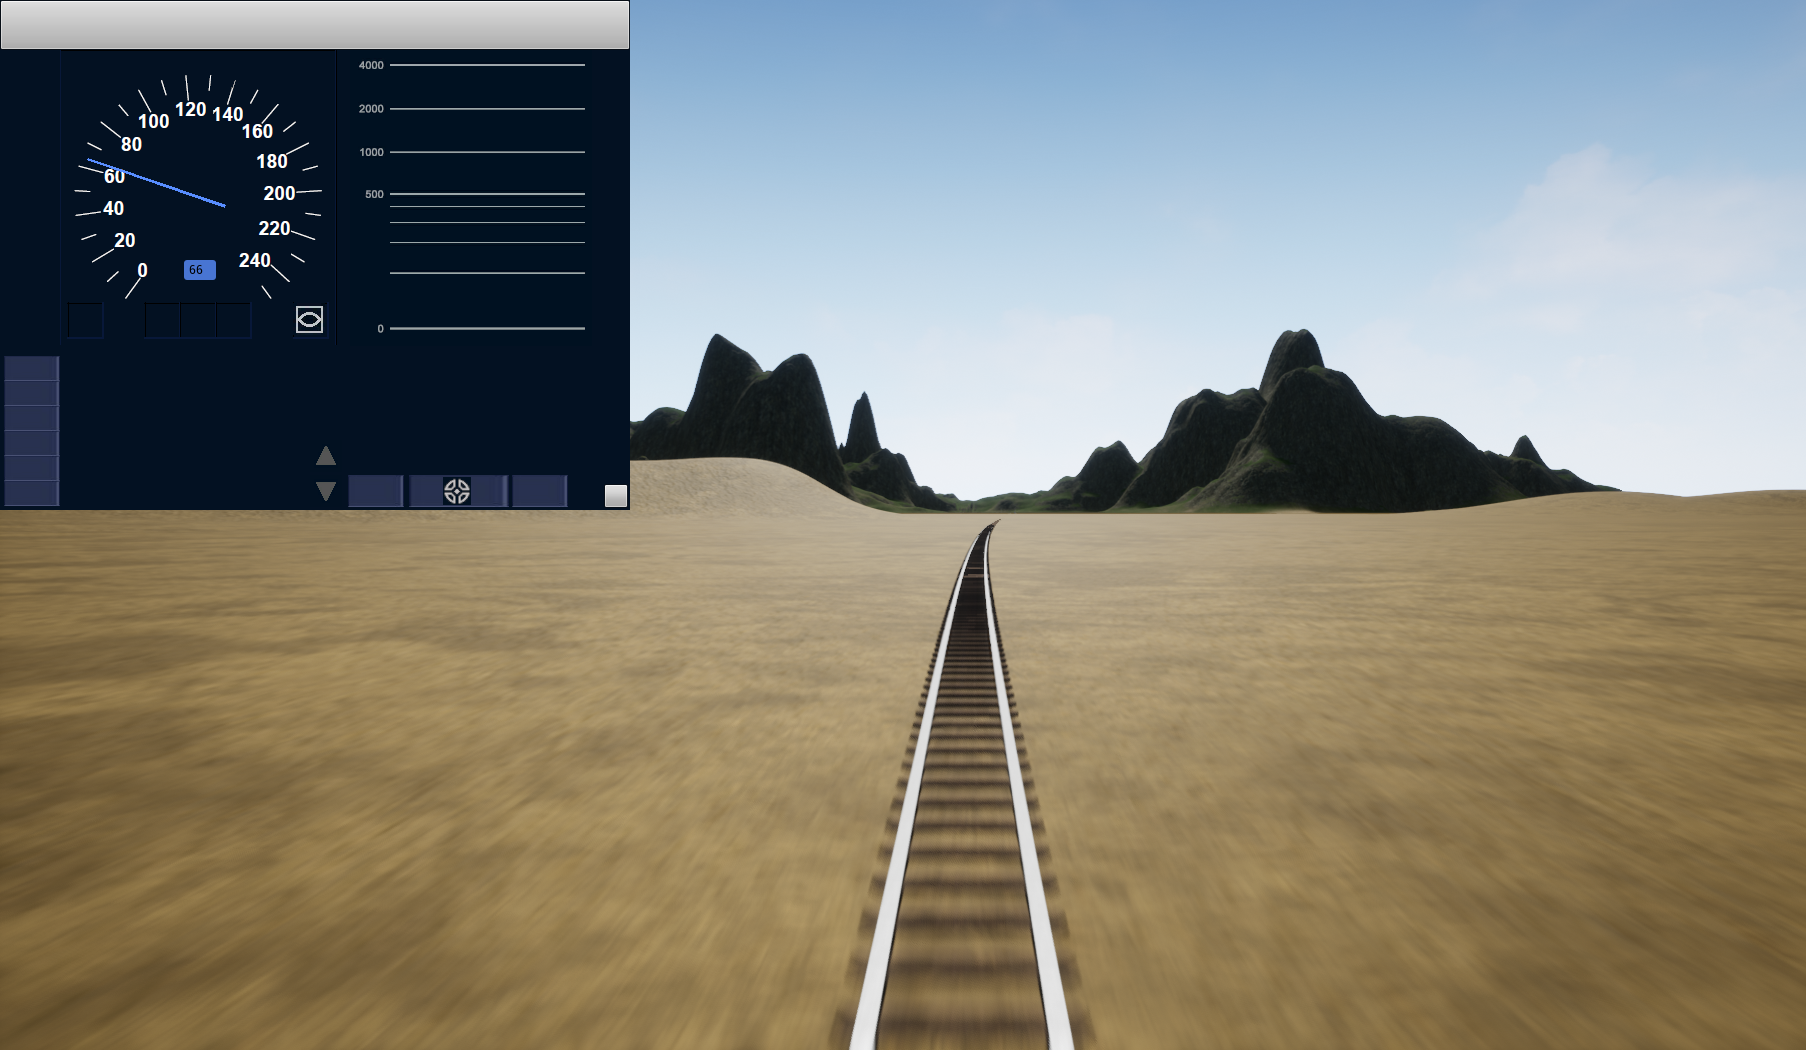
\includegraphics[width=0.8\textwidth]{figures/Tog Drive.PNG}
    %\vspace{-12pt}
    \caption{DeskSimV2: Train Driver View}
    \label{Train_Driver_View_img}
\end{figure}


The user will encounter different signals when running a level/scenario. The signal status and logic are pre-decided and controlled through invisible triggerboxes. These triggerboxes reacts to the position of the train and checks for certain conditions, and can update signal statuses accordingly. 

\begin{figure}[H]
    \centering

    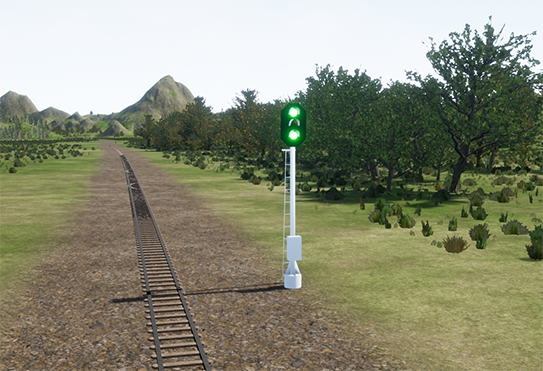
\includegraphics[width=6cm]{figures/Signal1.png}
    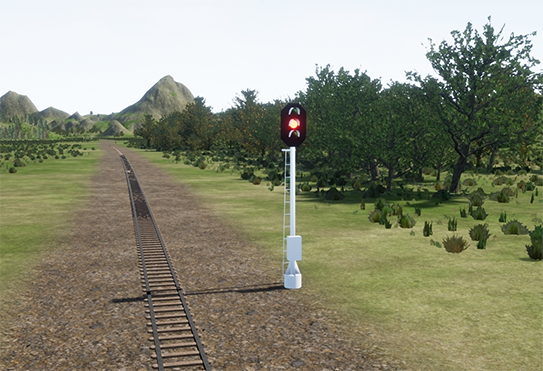
\includegraphics[width=6cm]{figures/Signal2.png}
    %\vspace{-12pt}
    \caption{DeskSimV2: Stop Signal}
    \label{Stop_Signal_img}
\end{figure} 


The simulator provides an option to the user where they can see the world in a drone mode, with free movement and camera rotation. The movement of the drone is independent of the train. 

\begin{figure}[H]
    \centering

    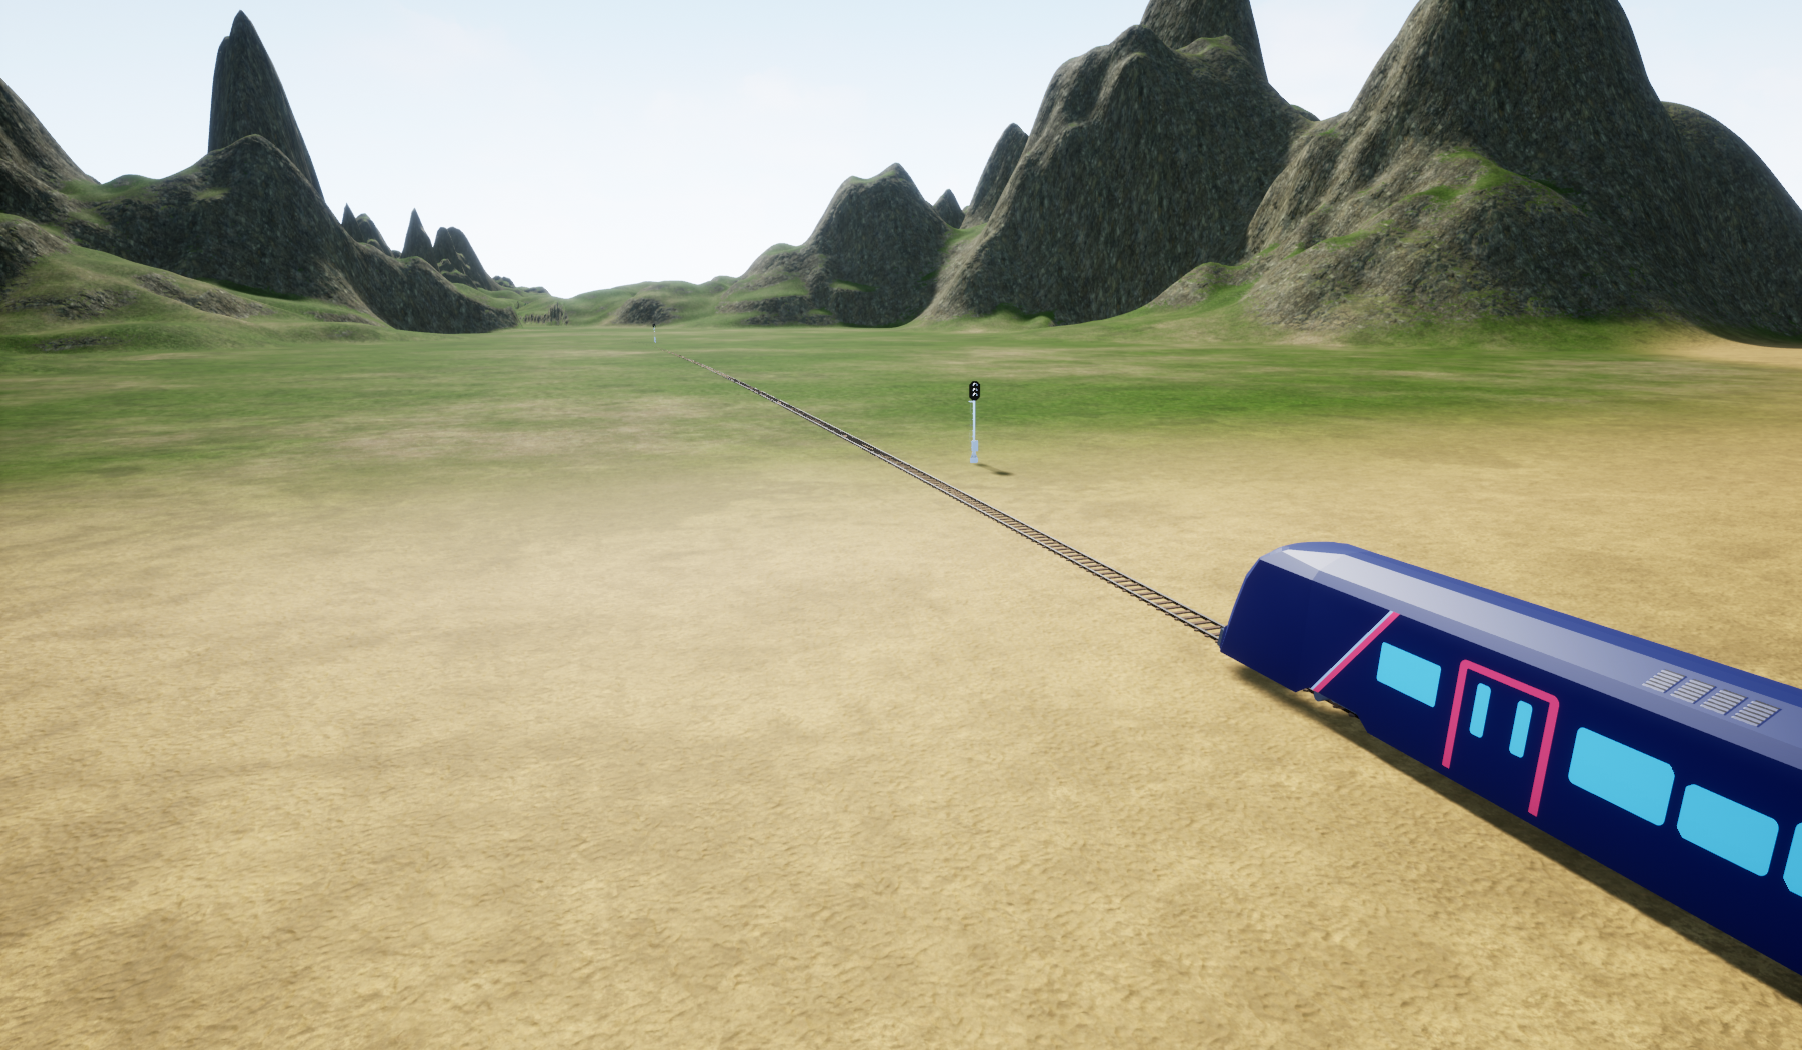
\includegraphics[width=6cm]{figures/DroneMode.PNG}
    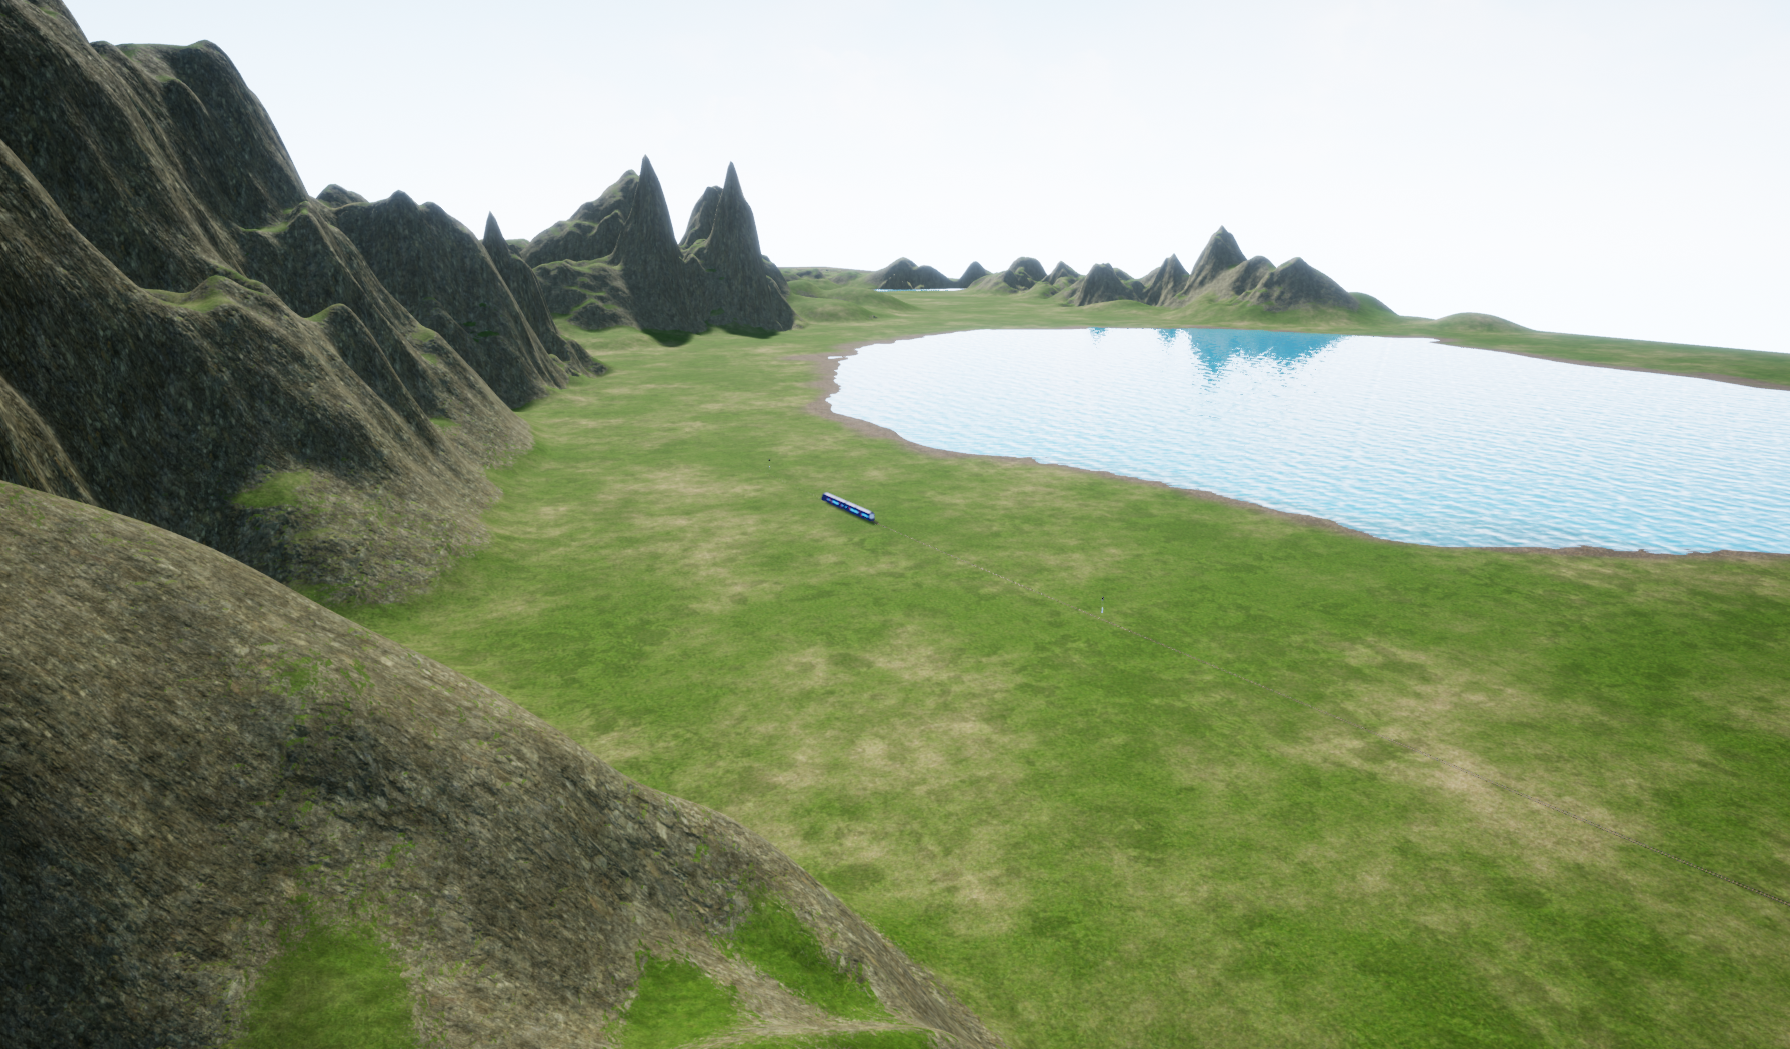
\includegraphics[width=6cm]{figures/DroneMode2.PNG}
    %\vspace{-12pt}
    \caption{DeskSimV2: Drone View}
    \label{Drone_Mode_img}
\end{figure} 

\section{Editor mode}

The editor mode has buttons presented on the top of the screen, where you can save your changes, change the current tool mode and delete objects. The editor mode interface also offers a window for adding new objects to the level. This is done by dragging the icon of the object and dropping it into the level.

\begin{figure}[H]
    \centering

    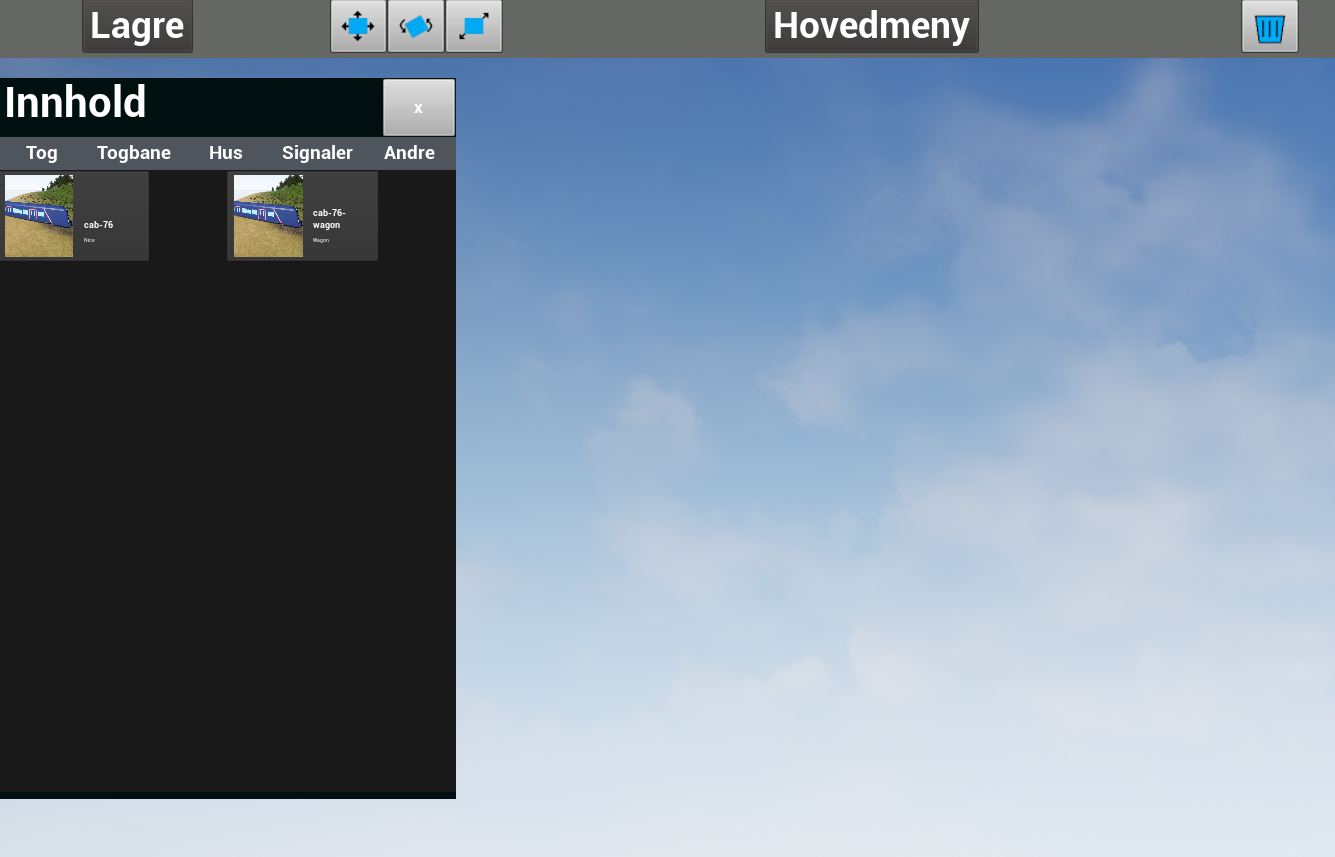
\includegraphics[width=0.9\textwidth]{figures/HUD1.png}
    %\vspace{-12pt}
    \caption{DeskSimV2: Editor Mode HUD}
    \label{Editor_Mode_img}
\end{figure} 